% Companion entry point for a separate supplementary PDF.
% CVPR 2027 Paper Template; see https://github.com/cvpr-org/author-kit

\documentclass[10pt,twocolumn,letterpaper]{article}

%%%%%%%%% PAPER TYPE  - PLEASE UPDATE FOR FINAL VERSION
% \usepackage{cvpr}              % To produce the CAMERA-READY version
\usepackage[review]{cvpr}      % To produce the REVIEW version
% \usepackage[pagenumbers]{cvpr} % To force page numbers, e.g. for an arXiv version

% Import additional packages in the preamble file, before hyperref
%% This file contains a number of tweaks that are typically applied to the main document.
%% They are not enabled by default, but can be enabled by uncommenting the relevant lines.

%%
%% Inline annotations; for predefined colors, refer to "dvipsnames" in the xcolor package:
%% https://tinyurl.com/overleaf-colors
%%
\newcommand{\red}[1]{{\color{red}#1}}
\newcommand{\todo}[1]{{\color{red}#1}}
\newcommand{\TODO}[1]{\textbf{\color{red}[TODO: #1]}}
%%
%% disable for camera ready / submission by uncommenting these lines  
%%
% \renewcommand{\TODO}[1]{}
% \renewcommand{\todo}[1]{#1}

%%
%% work harder in optimizing text layout. Typically shrinks text by 1/6 of page, enable
%% it at the very end of the writing process, when you are just above the page limit
%%
% \usepackage{microtype}

%%
%% fine-tune paragraph spacing
%%
% \renewcommand{\paragraph}[1]{\vspace{.5em}\noindent\textbf{#1.}}

%%
%% globally adjusts space between figure and caption
%%
% \setlength{\abovecaptionskip}{.5em}


%%
%% Allows "the use of \paper to refer to the project name"
%% with automatic management of space at the end of the word
%%
% \usepackage{xspace}
% \newcommand{\paper}{ProjectName\xspace}

%%
%% Commonly used math definitions
%%
% \DeclareMathOperator*{\argmin}{arg\,min}
% \DeclareMathOperator*{\argmax}{arg\,max}

%%
%% Tigthen underline
%%
% \usepackage{soul}
% \setuldepth{foobar}
% Additional packages required by the manuscript's existing tables.
\usepackage{float}
\usepackage{array}


% It is strongly recommended to use hyperref, especially for the review version.
% hyperref with option pagebackref eases the reviewers' job.
% Please disable hyperref *only* if you encounter grave issues, 
% e.g. with the file validation for the camera-ready version.
%
% If you comment hyperref and then uncomment it, you should delete *.aux before re-running LaTeX.
% (Or just hit 'q' on the first LaTeX run, let it finish, and you should be clear).
\definecolor{cvprblue}{rgb}{0.21,0.49,0.74}
\usepackage[pagebackref,breaklinks,colorlinks,allcolors=cvprblue]{hyperref}

\def\confName{CVPR}
\def\confYear{2027}

%%%%%%%%% TITLE - PLEASE UPDATE
\title{GeoGate: Evaluating Late-Layer Token Pruning in 3D Large Multimodal Models}

%%%%%%%%% AUTHORS - PLEASE UPDATE
\author{Anonymous Author(s)}

\begin{document}
\clearpage
\setcounter{page}{1}
\maketitlesupplementary

% Preserve the manuscript's appendix and S-number conventions.
\appendix
\setcounter{table}{0}
\setcounter{figure}{0}
\setcounter{equation}{0}
\renewcommand{\thetable}{S\arabic{table}}
\renewcommand{\thefigure}{S\arabic{figure}}
\renewcommand{\theequation}{S\arabic{equation}}
% Distinct destinations also support the template's optional combined build.
\renewcommand{\theHtable}{supp.\arabic{table}}
\renewcommand{\theHfigure}{supp.\arabic{figure}}
\renewcommand{\theHequation}{supp.\arabic{equation}}

\section*{Overview and reading guide}
\label{sec:supp_scope}

This supplement provides the protocols, controls, and additional results supporting the empirical study of GeoGate. We distinguish attention-pattern stability, selected-set relevance, retention quality, and measured efficiency. Each comparison uses its own matched inputs and native (unpruned) baseline.

\Cref{sec:supp_protocols} defines the experimental setup, implementation, and inference conventions. \Cref{sec:supp_profiles} examines attention profiles. \Cref{sec:supp_functional} compares complete-answer own-set deletion with fixed-set controls to distinguish token identity from deletion depth. \Cref{sec:supp_quality,sec:supp_transfer} distinguish development-set sensitivity from task transfer and external evaluation. \Cref{sec:supp_efficiency} separates analytical cost from measured time. \Crefrange{sec:supp_repro}{sec:supp_limitations} provide reproduction details, qualitative examples, and remaining validation requirements.

\section{Experimental setup and inference conventions}
\label{sec:supp_protocols}
The two model settings differ in representation as well as token count. LLaVA-3D-7B and 3D-LLaVA-7B-LoRA use approximately 1500 and 100 spatial tokens, respectively; model, representation, and training differences prevent a controlled token-count scaling interpretation.

GeoGate combines late-prefill pruning with all-layer prompt key--value (KV) cache compaction before decoding. L14 denotes a full zero-indexed block L14, followed by pruning before L15. The default relative budget ($R=0.10$) and fixed 128-token comparisons are distinct operating points. Quality and timing characterize the combined prefill/cache intervention.


\subsection{Models, inputs, and paired comparisons}
We report exact match (EM), consensus-based image description evaluation (CIDEr), and mean intersection over union (mIoU).
\Cref{tab:supp_protocolmap} identifies the principal ScanQA runners and their matching boundaries. Comparisons are paired within a row; estimates from different runners are not pooled. In particular, equal final token counts in the official 3DZip comparison do not imply equal total cost.
\begin{table*}[t]
\centering
\small
\setlength{\tabcolsep}{4pt}
\caption{Core LLaVA-3D ScanQA protocol map. These runners use the inspected ScanQA validation split: 4675 questions/71 scenes. Matching applies within a row, not across rows; --- means CIDEr is not reported for replay.}
\label{tab:supp_protocolmap}
\begin{tabular}{@{}p{0.17\textwidth}p{0.20\textwidth}p{0.14\textwidth}p{0.15\textwidth}p{0.25\textwidth}@{}}
\toprule
Runner & Intervention or budget & Matched within runner & Native EM/CIDEr & What the comparison establishes \\
\midrule
Schedule/scorer grid & Relative retention; default L14/$R=0.10$ & Inputs, prompt, decoding & 27.34/93.96 & Quality sensitivity on the development split; not independent preservation. \\
Analytical cost controls & L14/$K=128$; length-conditioned L2/L8 budgets & Prepared embedding, analytical LM cost & 27.42/94.06 & Selected early/late controls at matched analytical cost, not measured latency. \\
Official 3DZip comparison & 3DZip/$K=128$ and L14/$K=128$ & RGB-D, prompt, per-query seed & 27.23/93.48 & Quality at equal retained-token count; computation and latency are not matched. \\
Complete-answer deletion & Layer-specific top, random, bottom sets; fixed-set replay & Prepared embedding, deletion budget, baseline & 27.36/93.95 & Set-level relevance; fixed sets do not support an L14-specific damage maximum. \\
Shared-input layer replay & Relative retention; $R=0.10$ across 11 pruning layers & Video tensor, expanded embedding, per-query seed & 27.4225/--- & Layer means and simultaneous contrasts; no resolved superiority over native or adjacent late settings. \\
\bottomrule
\end{tabular}
\end{table*}

LLaVA-3D QA uses the suffix ``Answer the question simply.'' and self-sampled stride-10 frames. The schedule-grid native baseline is 27.34 EM/93.96 CIDEr. A separate beam-5 diagnostic gives 27.40/100.86, demonstrating decoding sensitivity while leaving the difference from published results unresolved. LLaVA-3D SQA3D changes EM from 55.90 to 55.53 (scene 95\% CI $[-0.87,0.14]$). On 3D-LLaVA ScanQA, retaining 50, 25, and 10 of 100 superpoints gives 28.04, 27.94, and 27.83 EM, versus 27.87 native. Each result retains its runner-specific protocol. The 500-question exploratory subset samples one question per scene, then adds questions round-robin across all 71 scenes. This ensures scene coverage without guaranteeing coverage of every semantic scene type.

\subsection{Pruning, cache compaction, and decoding}
\label{sec:supp_implementation}
\paragraph{KV index mapping.} Layers through the pruning block cache the full sequence; later layers cache the reduced sequence. GeoGate records the original-position map at each resulting length and slices every layer's cache to the final kept set. The map starts in original sequence order and is updated with kept indices after each drop. Each layer searches its saved map for the final original positions to obtain the key/value slice. We check that mappings are valid, sorted, and unique, and that cache lengths agree before decoding. This synchronization supports the tested interface's common 4D decode mask; other pruning interfaces need not impose this constraint. Early-layer prompt caches are also compacted despite their full-length prefill computation. The reported prompt-KV reduction depends on this all-layer operation, whose quality and timing effects were not isolated from late-prefill pruning.

For a layer with cache length $\ell_i$, let $M_{\ell_i}$ be its saved original-position map and $M_{T_{\text{kept}}}$ the final kept map. The cache-slicing index expression is
\begin{equation}
\mathcal{J}_i \;=\; \operatorname{searchsorted}\!\big(M_{\ell_i},\; M_{T_{\text{kept}}}\big),
\end{equation}
and is applied to both key and value tensors. Eager attention is configured before the L14 forward; the scorer reads that same forward's attention weights, without an additional L14 pass.

\paragraph{Single-token decode.} After cache pruning, the original attention mask can be longer than the cache. The tested HuggingFace input-preparation path can consequently feed multiple tokens per decode step. GeoGate restricts input to the final token and rebuilds the mask from actual cache length. Full-generation checks verify one-token forwards and monotonic KV growth. Without this correction, mask-minus-cache input preparation can repeatedly re-feed generated tokens, increasing latency. Continued re-feeding can exceed the supported position range for rotary position embeddings (RoPE). The tested generation path implements the correction by wrapping \texttt{prepare\_inputs\_for\_generation}.

\paragraph{RoPE positions.} Retained spatial tokens keep their original position IDs. A 500-question pilot shows that compact re-indexing changes EM from 30.80 to 18.20 and produces truncated answers. This result motivates the position-preservation invariant without identifying a uniquely 3D positional mechanism.

\paragraph{Deterministic scene cap.} Three ScanQA scenes exceed the 2,560-token preparation cap. We reuse a deterministic scene-level CPU permutation across slots, conditions, and processes. Cap summaries and selected-index hashes reproduce across all three tensor-batch sessions. Independent slot-level caps would assign different spatial evidence to duplicated inputs. The shared permutation instead depends on scene identity, seed, and pre-cap count. It controls input construction separately from GeoGate's attention ranking.

\subsection{Statistical estimands and inference scope}
\label{sec:supp_statistics}

Quality differences are paired within a runner. EM and mIoU use 0--100 scales, while CIDEr differences use score points. Scene bootstrap samples scene labels with replacement, includes all paired questions from each sampled scene, and computes a question-weighted mean. CIDEr resampling holds reference-corpus inverse document frequency (IDF) contributions fixed. Question-level and scene-level intervals target different resampling units and are labeled separately.

Two-sided central 95\% percentile intervals use the 2.5th and 97.5th percentiles. The prespecified two-sided 97.5\% intervention and cost-control intervals instead use the 1.25th and 98.75th percentiles. These are not one-sided 97.5\% lower bounds. The SQA3D and MMScan quality gates use the lower endpoint of a two-sided 95\% interval as the one-sided 97.5\% bound. Simultaneous max-$t$ intervals apply only to their stated comparison family; the five-benchmark Holm analysis retains marginal percentile intervals and adjusts the endpoint $p$-values separately.

ScanQA validation informed configuration selection. Analyses on that split remain conditional on selection unless explicitly stated otherwise, even when individual comparisons were specified before their outputs. Leave-one-scene-out selection and bootstrap-seed checks assess stability within this development setting, not independent confirmation. An interval containing zero does not by itself establish equivalence or non-inferiority; either claim requires a prespecified margin and an appropriate decision rule. These limitations apply throughout the sensitivity analyses; individual sections identify additional confounds.

The original per-endpoint quality report uses 10,000 draws and seed 20260904. Earlier protocol summaries record 20260906 for B1 latency, 20260912 for tensor-batch throughput, and 20260913 for the two LLaVA-3D interventions. Follow-ups retain their indexed run-specific seeds. Random-arm inference conditions on the three frozen rankings, not an unlimited population of random sets.

\subsection{Selection and evaluation chronology}
\label{sec:supp_selection}

The layer and relative budget were selected using inspected ScanQA validation point estimates. The profile-derived onset window and threshold were also chosen after inspecting the profiles. These early choices precede the later controlled comparisons, but available records do not reconstruct every early search decision or a complete timestamp chain.

The fixed-token-set control followed the own-set deletion results that exposed the identity--depth confound. Its protocol specified the comparison before the fixed-set outputs, but reuse of the split keeps the result conditional on development. \Cref{sec:supp_sqa_validation} details the sequential SQA3D fold design. The MMScan protocol specified its subset and superiority criterion before MMScan outputs. Budget follow-ups, profile-to-quality coupling, and throughput mismatch exclusions are post-hoc analyses. \Cref{sec:supp_repro_index} indexes the protocols and source records.

\section{Attention profiles and stability}
\label{sec:supp_profiles}

We examine whether the observed attention pattern persists across samples and prompts. These analyses characterize attention allocation; separate retention experiments assess its relevance to pruning quality.

\paragraph{Attention-statistic definitions.} Spatial attention mass and half-mass coverage use the last-prompt query row of head-averaged prefill attention. Received-attention Gini instead sums all prefill query rows for each spatial key before sorting the keys. Its denominator includes the frozen $10^{-9}$ stabilization term. For each sample, heads are averaged before computing these statistics; sample-level statistics are then averaged at each layer. Gini therefore measures inequality in all-query received attention, which need not track concentration in the last-prompt readout.



\subsection{Late-layer summary statistics}
\Cref{tab:supp_profile_statistics} reports aggregate 50-scene profiles separately from question-level profiles. Aggregate entries are ranges of L14--L26 layer means, rather than uncertainty intervals. Question-level entries first average each question over L14--L26, then use a scene-cluster bootstrap to obtain a 95\% interval over questions. Half-mass coverage is the spatial-token fraction covering 50\% of a layer's last-prompt spatial attention mass.

\begin{table*}[t]
\centering
\small
\caption{Frozen spatial-attention statistics for L14--L26. Aggregate rows report layer-mean ranges; question rows report question-level phase means with scene-cluster 95\% intervals.}
\label{tab:supp_profile_statistics}
\begin{tabular}{lcccc}
\toprule
Profile & Items & Late attention & Half-mass coverage & Tokens \\
\midrule
LLaVA-3D, 50 scenes & 50 & 7.58--23.02\% & 2.21--5.76\% & 33.2--86.3 \\
3D-LLaVA, 50 scenes & 50 & 4.73--14.29\% & 4.68--11.58\% & 4.7--11.6 \\
LLaVA-3D, 200 q. & 200/67 & 15.21 [14.33,16.10]\% &
3.97 [3.71,4.23]\% & 55.7 [49.4,62.1] \\
3D-LLaVA, 71 scenes & 71/71 & 9.70 [8.69,10.72]\% &
5.81 [5.21,6.44]\% & 5.8 [5.2,6.4] \\
\bottomrule
\end{tabular}
\end{table*}

The 50-scene and question-level profiles use different samples, so their ranges cannot be pooled. These intervals characterize the inspected profiles without establishing a universal layer or mechanism.

\subsection{Prompt perturbations}
The L14 readout resurgence persists under the tested answer-format changes. We use the frozen 200-question profile across 67 scenes with three prompts: the original, removal of its suffix, and the paraphrase ``Give a short answer.'' \Cref{tab:supp_prompt} reports scene-clustered bootstrap intervals. The L14--L13 attention jump remains positive for all three prompts, and the retained top-10\% set at L14 strongly overlaps the original-prompt set. This supports directional stability under two fixed perturbations, without establishing invariance to arbitrary prompts.

\begin{table}[t]
\centering
\caption{Prompt perturbation of the L14 readout profile.}
\label{tab:supp_prompt}
\resizebox{\columnwidth}{!}{%
\begin{tabular}{lcc}
\toprule
Prompt & L14--L13 jump (95\% CI) & Top-set overlap (95\% CI) \\
\midrule
Original & 10.56 [9.77, 11.36] & 1.000 \\
No suffix & 5.08 [4.33, 5.82] & 0.892 [0.887, 0.898] \\
Paraphrased suffix & 9.11 [8.36, 9.86] & 0.952 [0.948, 0.955] \\
\bottomrule
\end{tabular}}
\end{table}

\subsection{Profile-derived onset rule}
A retrospective label-free rule identifies a stable onset in the model-level mean profiles. Using the recorded per-sample profiles, it scans L2--L31 and takes the late peak over L14--L26. It selects the first layer in L2--L31 whose mean last-prompt-to-spatial attention reaches 50\% of that peak. The rule selects L14 in both architectures. Recomputing the mean curve while leaving out each scene still selects L14 in 67/67 LLaVA-3D scenes and 71/71 3D-LLaVA scenes. A 10,000-draw scene bootstrap also selects L14 in 10,000/10,000 resamples for both profiles.

The late peaks occur at L24 and L21, so the rule identifies an onset rather than the maximum. Threshold sensitivity remains descriptive: 30\% selects L9 and L11, 40--60\% selects L14 in both profiles, and 70\% selects L14 and L17. Per-question selections vary across layers. The result therefore supports a reproducible model-level heuristic, without per-question adaptivity or a universal L14 boundary. The reference peak window and threshold were chosen after profile inspection, so phase discovery is not independent.

\subsection{Question-type coverage}
Spatial, counting, and residual ``other'' questions have wider mean readout sets than color questions in the frozen 200-question LLaVA-3D profile (\Cref{tab:supp_qtype}). This pattern is descriptive: counting has only ten examples, and full-set correctness analysis shows no corresponding concentration of GeoGate errors.

\begin{table}[t]
\centering
\caption{LLaVA-3D readout coverage by ScanQA question type.}
\label{tab:supp_qtype}
\begin{tabular}{lcc}
\toprule
Type & Questions & Top-50 coverage \\
\midrule
Color & 36 & 2.53\% \\
What-object & 45 & 3.46\% \\
Spatial relations & 88 & 4.55\% \\
Counting & 10 & 4.06\% \\
Other & 21 & 5.02\% \\
\bottomrule
\end{tabular}
\end{table}

\section{Token-set relevance and deletion location}
\label{sec:supp_functional}
We assess selected-set relevance while distinguishing token identity from deletion depth. Complete-answer own-set deletion on LLaVA-3D establishes the initial comparison; fixed-set deletion then tests its depth interpretation. Retention tests, first-token responses, and diagnostic analyses provide complementary evidence.


\subsection{Intervention effects and interval conventions}
\label{sec:supp_damage}

We distinguish deletion damage, extra damage relative to random deletion, and cross-layer differences. Let $Q_i^0$ be the native score for question $i$, and $Q_i(S,\ell)$ its score after deleting set $S$ at layer $\ell$. The basic deletion damage is
\begin{equation}
D_i(S,\ell)=Q_i^0-Q_i(S,\ell).
\end{equation}
For first-token tests, $Q_i$ is the log probability of the native argmax answer token. For complete-answer tests, it is EM on the 0--100 scale or the per-query CIDEr contribution with the reference corpus fixed. The additional damage of the top-attended set relative to the frozen random sets is
\begin{equation}
E_i(\ell)=D_i(S_{\ell}^{\rm top},\ell)
-\frac{1}{3}\sum_{r=1}^{3}D_i(S_{\ell,r}^{\rm random},\ell).
\end{equation}
Thus, positive extra EM damage equals random-deletion EM minus top-deletion EM. Own-set cross-layer contrasts compare $E_i(14)$ with $E_i(8)$ or $E_i(20)$; token identities can differ across layers. The fixed-set control instead holds one source set $S_s$ constant and compares $D_i(S_s,14)$ with $D_i(S_s,8)$ or $D_i(S_s,20)$. Because these contrasts use basic damage $D$ rather than random-adjusted extra damage $E$, subtracting the two contrast estimates does not isolate the contribution of token identity. Retention tests compare retained-set quality directly and do not follow from deletion damage alone.

Intervention contrasts use two-sided central 97.5\% scene-bootstrap intervals, following \cref{sec:supp_statistics}. Supporting within-layer effects use 95\% intervals where stated. Random-arm $\pm$ values are sample standard deviations across the three recorded rankings.

\subsection{LLaVA-3D complete-answer deletion}
Complete-answer deletion tests whether each layer's top-attended set matters more than matched random or bottom-attention sets. The evaluation covers 4,675 questions from 71 scenes under 16 conditions. All arms share prepared multimodal inputs and preserve text tokens, one-token decode updates, and monotonic KV growth at every layer. \Cref{tab:supp_generation} reports the answer-level effects.

\begin{table*}[t]
\centering
\small
\caption{Complete-answer deletion on LLaVA-3D ScanQA. Extra damage is mean random-deletion score minus top-deletion score, expressed in EM points or CIDEr score points.}
\label{tab:supp_generation}
\begin{tabular}{lccccc}
\toprule
Layer & Top EM & Random EM & Bottom EM & Extra EM damage & Extra CIDEr damage \\
\midrule
L8 & 27.04 & 27.32 & 27.36 & 0.29 & 1.21 \\
L14 & 23.87 & 27.36 & 27.29 & 3.49 & 10.52 \\
L20 & 26.87 & 27.38 & 27.38 & 0.51 & 2.59 \\
\bottomrule
\end{tabular}
\end{table*}

For the previously selected L14/10\% configuration, both prespecified cross-layer damage contrasts are positive. L14-minus-L8 and L14-minus-L20 are 3.20 [1.80, 4.73] and 2.97 [1.83, 4.22] EM points, respectively, with 97.5\% scene-clustered intervals. The supporting L14 top-minus-bottom contrast is 3.42 [2.31, 4.59], with a 95\% interval. CIDEr shows the same ordering. These results support selected-set relevance without establishing individual-token causality.

\subsection{Fixed-token-set cross-layer control}
\label{sec:supp_fixed_control}
The own-set comparison changes token identities together with deletion depth. The fixed-set control varies deletion depth while holding token identity constant. Each source layer's top-attention set is replayed at L8, L14, and L20. It matches the complete-answer runner's 4,675 questions, 71 scenes, prepared inputs, baseline, prompt, deletion budget, and seed. Unpruned outputs reproduce the complete-answer baseline exactly. The prespecified rule requires both L14-over-L8 and L14-over-L20 EM-damage contrasts to have 97.5\% scene-bootstrap lower bounds above zero. At least two of the three source sets must meet both conditions.

\begin{table}[t]
\centering
\caption{Fixed-token-set cross-layer deletion on LLaVA-3D. Basic damage is native minus deletion-condition EM. Each contrast holds the source set fixed; positive values indicate greater damage at L14. Brackets are two-sided central 97.5\% scene-bootstrap intervals.}
\label{tab:supp_fixed_set}
\resizebox{\columnwidth}{!}{%
\begin{tabular}{lcc}
\toprule
Source set & L14 minus L8 & L14 minus L20 \\
\midrule
L8  & $-0.26$ $[-0.70,0.19]$ & $+0.15$ $[-0.19,0.51]$ \\
L14 & $-1.50$ $[-2.29,-0.70]$ & $+2.63$ $[1.60,3.77]$ \\
L20 & $-1.30$ $[-2.03,-0.59]$ & $+2.16$ $[1.29,3.15]$ \\
\bottomrule
\end{tabular}}
\end{table}

For both late-derived source sets, damage decreases from L8 to L14 to L20 (\Cref{tab:supp_fixed_set}). Neither contrast is resolved for the L8-derived set. Zero of three source sets supports both required directions, so the prespecified criterion is not met.

These results do not support L14 as a location-specific damage maximum for the late-derived sets. They retain evidence that deletion depth matters in these comparisons, while limiting a location-only explanation of the own-set L14 peak. The own-set contrasts use extra damage $E$; the fixed-set contrasts use basic damage $D$ (\cref{sec:supp_damage}). Their numerical difference is not a pure token-identity effect. Neither set-level intervention establishes individual-token causality or the sufficiency of retaining only the selected 10\%.

A secondary balanced factorial decomposition summarizes variation across the same nine cell means. Source-set identity accounts for $49.9\%$ of between-cell variation (95\% scene-bootstrap interval $[37.9,59.6]$), prune layer for $36.4\%$ $[28.0,46.7]$, and their interaction residual for $13.7\%$ $[10.5,17.9]$. These shares describe the nine-cell mean matrix, not causal contributions to question-level error. The interaction share is a ratio of squared residuals and is nonnegative by construction. Its positive percentile interval therefore does not test a zero-interaction null. Such inference would require signed interaction contrasts or a null-calibrated joint test, with appropriate comparison-family correction. We use this post-hoc decomposition descriptively, without a significance or causal-attribution claim. It cannot alter the failed prespecified L14-location gate or establish an L14-specific damage maximum.

\subsection{3D-LLaVA retention and deletion}
Bidirectional interventions test selected-set relevance in 3D-LLaVA's 100 superpoint tokens. At L14, retaining ten top-attended tokens gives higher scores than random or bottom retention. Deleting that set causes more damage than deleting either control (\Cref{tab:supp_bidir}). Random-control values report means and sample standard deviations over seeds 101, 202, and 303. The retention arm removes the other 90 tokens; the deletion arm keeps them. These complementary interventions therefore test different questions: deletion relevance does not establish retention sufficiency or equivalence to unpruned generation.

\begin{table}[t]
\centering
\caption{Bidirectional L14 intervention on 3D-LLaVA ScanQA.}
\label{tab:supp_bidir}
\resizebox{\columnwidth}{!}{%
\begin{tabular}{lcccc}
\toprule
& \multicolumn{2}{c}{Retain 10} & \multicolumn{2}{c}{Delete 10} \\
\cmidrule(lr){2-3}\cmidrule(lr){4-5}
Set & EM@1 & CIDEr & EM@1 & CIDEr \\
\midrule
Top attention & 27.83 & 90.42 & 23.81 & 78.95 \\
Random & $23.87\pm0.07$ & $78.52\pm0.73$ &
         $27.79\pm0.12$ & $89.36\pm0.39$ \\
Bottom attention & 23.51 & 78.12 & 28.09 & 90.16 \\
\bottomrule
\end{tabular}}
\end{table}

The separate frozen cross-layer runner confirms higher scores for top retention at all three layers (\Cref{tab:supp_stage}). L14 has the largest deletion-damage point estimate, but its retention contrast against L8 is unresolved at the prespecified level. The two intervention directions therefore do not uniquely identify L14 in every comparison.

Question-level results show stronger agreement for L14 versus L20. L14-minus-L20 is positive in both frozen directions: deletion damage is 2.62 [1.66, 3.59] and retention gain is 2.92 [1.90, 4.07], with 97.5\% scene-clustered intervals. Among 229 questions with nonzero effects in both directions, 150 favor L14 in both and 52 favor L20 in both. Thus, 202/229 (88.2\%) pairs agree in sign. The remaining 11 pairs favor L14 only under deletion, and 16 only under retention. Scene-bootstrap Pearson and Spearman correlations are 0.430 [0.371, 0.484] and 0.375 [0.319, 0.429]. L14-minus-L8 is positive under deletion, 1.71 [0.52, 2.99], but unresolved under retention, 1.04 $[-0.15, 2.21]$. We therefore distinguish the cross-direction L14-versus-L20 result from the deletion-only L14-versus-L8 result. Both runs reuse the inspected ScanQA validation split and provide complementary controls, not independent replications.



\begin{table*}[t]
\centering
\caption{Cross-layer retention and deletion on 3D-LLaVA. Random arms average three frozen seeds.}
\label{tab:supp_stage}
\begin{tabular}{lcccccc}
\toprule
& \multicolumn{3}{c}{Retain 10} & \multicolumn{3}{c}{Delete 10} \\
\cmidrule(lr){2-4}\cmidrule(lr){5-7}
Layer & Top & Random & Bottom & Top & Random & Bottom \\
\midrule
L8 & 25.28 & 22.28 & 21.37 & 25.71 & 28.04 & 28.04 \\
L14 & 27.81 & 23.76 & 23.53 & 23.89 & 27.93 & 28.11 \\
L20 & 27.76 & 26.64 & 26.12 & 26.57 & 27.99 & 28.09 \\
\bottomrule
\end{tabular}
\end{table*}

\subsection{LLaVA-3D first-token response}
A separate label-free endpoint measures the first answer token's response to deletion, complementing the complete-answer analysis. Damage measures the decrease in the native baseline argmax token's log probability after deleting a matched 10\% spatial-token set. \Cref{tab:supp_firsttoken} reports the difference between top-attention and random deletion damage.

\begin{table}[t]
\centering
\caption{First-token extra deletion damage on LLaVA-3D ScanQA: top-attention minus mean random-control damage, in log-probability units. Intervals are two-sided central 95\% scene-bootstrap intervals.}
\label{tab:supp_firsttoken}
\begin{tabular}{lcc}
\toprule
Layer & Extra log-prob. damage & Scene 95\% CI \\
\midrule
L8 & 0.029 & [0.016, 0.044] \\
L14 & 0.280 & [0.241, 0.324] \\
L20 & 0.064 & [0.053, 0.077] \\
\bottomrule
\end{tabular}
\end{table}

Both prespecified cross-layer contrasts are positive under 97.5\% scene intervals: L14-minus-L8 is 0.251 [0.212, 0.296], and L14-minus-L20 is 0.216 [0.180, 0.257]. The supporting L14 top-minus-bottom contrast is 0.282 [0.242, 0.326], with a 95\% interval. Argmax flips, margin damage, Jensen--Shannon divergence, and final-prompt hidden-state displacement show the same ordering. Because native and intervention arms use different forward paths, we interpret within-layer top-minus-control effects and their cross-layer differences.

The first-token and complete-answer runners share baseline, top-attention, and bottom-attention token sets for all 4,675 questions at all three layers. Random controls use separate frozen namespaces, so we do not pool their draws across endpoints. Mean Jaccard overlap between top-deleted sets is 0.207 [0.200, 0.215] for L8--L14, 0.417 [0.408, 0.426] for L14--L20, and 0.200 [0.192, 0.209] for L8--L20. Deterministic contrasts thus share inputs across endpoints, but selected sets differ across layers. Cross-layer deletion alone cannot separate pruning depth from token-set identity; \Cref{sec:supp_fixed_control} tests this confound with fixed token sets.

\subsection{Token-set overlap diagnostics}
We next stratify questions by deletion-set overlap to assess whether the layer contrasts persist when compared sets are most similar. Within the highest-overlap quartile, L14-minus-L8 complete-answer damage is $0.998$ EM points, with an exploratory 95\% scene interval $[-0.919,2.929]$ crossing zero. L14-minus-L20 remains positive at $4.277$ EM points $[2.415,6.343]$. Neither contrast varies monotonically across overlap quartiles. Because this post-hoc stratification uses the inspected split, it remains descriptive rather than causal. It provides weaker depth evidence for L14 versus L8 than for L14 versus L20.

Post-hoc overlap stratification shows the same limitation in the 3D-LLaVA deletion endpoint. Within the highest-overlap quartile (1,169 questions), L14-minus-L8 falls to 0.94 EM points, with an exploratory 95\% scene interval $[-1.35,3.32]$ crossing zero. L14-minus-L20 remains positive at 2.88 EM points $[1.11,4.63]$. Conditioning on token-set similarity therefore weakens the L14-versus-L8 evidence on this inspected split. This descriptive stratification does not provide a causal decomposition or replace the fixed-token-set control.

\subsection{Question dependence and semantic alignment}
The original-condition 200-question profile also permits a label-free comparison of top-10\% token sets across questions. At L14, mean Jaccard overlap is 0.245 [0.216, 0.274] within ScanQA scenes, versus 0.035 [0.033, 0.036] across scenes and an independent-subset chance mean of 0.053. Selected sets therefore contain a scene-linked component, while within-scene overlap remains far below one. However, visual embeddings are not hash-identical across all questions within each scene. This comparison cannot separate scene identity from frame sampling or question-conditioned processing, nor establish question-invariant anchors or an attention-sink mechanism.

The shared-input complete-answer run controls this visual-sampling confound. Across 4,675 questions in 71 scenes, each scene reuses identical raw RGB-D tensor hashes and a shared deterministic-cap fingerprint. L14 sets still vary substantially across questions within a scene: mean pairwise Jaccard overlap is 0.206 [0.196, 0.217], compared with 0.719 [0.704, 0.733] at L8 and 0.293 [0.279, 0.308] at L20. The independent-subset chance mean is 0.053. Under fixed scene inputs and cap choices, selection therefore contains a question-conditioned component rather than a single fixed anchor. This structural result does not establish semantic correctness, causal necessity, or a phenomenon unique to 3D inputs.

A voxel-to-label analysis tests semantic alignment with scene instances using the same 71 scenes and 4,675 frozen v15 questions. We map selected voxels to released ScanNet points through a fixed inverse axis-alignment transform and a 0.25 m radius. Mapping coverage is usable: the median mapped-token fraction is 0.9354 and median voxel-label purity is 0.9476. Nevertheless, the prespecified primary contrast fails. The L14 top-minus-random difference in instance foreground fraction is $-0.0070$, with a 95\% scene-clustered interval $[-0.0148,0.0007]$. The secondary labeled-semantic-presence difference is $+0.0241$ $[0.0117,0.0369]$ and cannot override that failure. We therefore retain selected-set relevance without claiming semantic identity or correctness, individual-token causality, or uniqueness to 3D inputs.

\subsection{Own-set robustness diagnostics}
These diagnostics assess the stability of the v15 own-set contrasts on the inspected split. They are separate from the v21 fixed-set analysis and do not alter its failed location criterion.

\paragraph{Scene and question-type variation.} Scene-level analysis shows that the own-set effects are not concentrated in a single observed scene. We recompute frozen v15 contrasts after subtracting each layer's three-seed random-control mean. L14 has greater extra damage than L8 in 47 of 71 scene means and than L20 in 49 of 71. The respective comparators lead in 16 and 14 scenes, with eight ties in each comparison. All 71 leave-one-scene-out estimates remain positive: 2.96--3.38 EM points for L14-minus-L8 and 2.79--3.14 for L14-minus-L20. Exact sign tests over discordant questions yield two-sided $p=1.19\times10^{-13}$ and $p=3.11\times10^{-13}$. These robustness results remain conditional on the inspected ScanQA validation split.

Exploratory question-type analysis finds positive contrasts across several categories, rather than a single heuristic type. With 95\% scene-clustered intervals, L14-minus-L8 extra damage is 2.78 [1.50, 4.17] EM points for spatial, 9.25 [4.47, 14.53] for color, and 2.80 [0.59, 4.85] for object questions. L14-minus-L20 gives 2.49 [1.25, 3.77], 9.82 [5.98, 14.09], and 2.09 [0.38, 3.80] for the same categories. Counting questions give $-0.88$ $[-4.82, 2.54]$ and $-0.29$ $[-2.45, 2.16]$; the residual ``other'' category also has intervals crossing zero. This post-hoc analysis uses imbalanced categories and provides neither a new prespecified test family nor independent confirmation.

A stricter descriptive comparison counts cases where the baseline is correct, top deletion is wrong, and at least two of three fixed random deletions remain correct. It yields 63, 273, and 106 cases at L8, L14, and L20, respectively. L14 has the largest count, but cases are selected post hoc from inspected validation. The counts therefore provide neither prevalence estimates nor causal token analysis.

\paragraph{Agreement across endpoints.} The two functional endpoints also agree in direction when paired across the same 4,675 questions. L14-minus-L8 is $0.2513$ $[0.2169,0.2898]$ in first-token log-probability damage and $3.20$ $[1.96,4.49]$ EM points in complete-answer damage. L14-minus-L20 is $0.2159$ $[0.1837,0.2512]$ and $2.97$ $[1.98,4.07]$, respectively. Among questions with nonzero effects in both endpoints, signs agree in 68.5\% and 69.1\% of cases. Scene-bootstrap Pearson correlations are $0.187$ $[0.113,0.268]$ and $0.187$ $[0.118,0.262]$. These zero-inflated question-level statistics support consistency across readouts, not individual-token causality or a complete decoding mechanism. Because the v21 fixed-token-set control does not reproduce both location contrasts for any source set, these results do not isolate an L14-specific maximum caused by deletion location alone.

\paragraph{Restricted layer-selection stability.} Nested scene-level selection assesses the stability of choosing L14. For each held-out scene, we select among three frozen candidate layers using the other 70 scenes, then evaluate that choice on the held-out scene. The first-token endpoint chooses L14 in 71/71 folds, with held-out damage $0.2800$ $[0.2405,0.3235]$. The complete-answer endpoint also chooses L14 in 71/71 folds, with $3.4866$ $[2.3567,4.6825]$ EM points of damage. Both endpoints select the same layer and agree on all three pairwise layer orderings in 71/71 folds. Candidate layers remain restricted to L8/L14/L20. This restricted candidate comparison does not establish a universal onset.

\section{Retention quality and design sensitivity}
\label{sec:supp_quality}
We examine how pruning layer, retention budget, and scoring rule affect quality on the inspected ScanQA split. Replay and sensitivity analyses assess these choices within the development setting. Selection stability and local multiplicity corrections neither provide independent confirmation nor account for the complete historical search.


\subsection{Schedule controls}
The schedule grid includes FastV-style L2/R10, PyramidDrop-style drops at L8/16/24 with cumulative ratios 0.50/0.25/0.125, and an AdaToken-inspired exponential-decay approximation. EM values are 23.04, 27.25, and 26.95, respectively, versus 27.79 for GeoGate.

The main-text FastV-style comparison instead uses L2/R50. Its GeoGate-minus-control scene intervals are $[0.55,2.02]$ EM and $[2.06,5.87]$ CIDEr. For PyramidDrop, the corresponding intervals are $[0.00,1.12]$ and $[-1.29,2.31]$; for AdaToken, they are $[0.29,1.41]$ and $[-0.01,2.98]$. These are implemented schedule controls rather than official reproductions. Relative to native, the headline R10 question-level EM interval is $[-0.02,0.92]$, with 77 wins, 4542 ties, and 56 losses.

\Cref{sec:supp_baseline_availability} documents related implementation availability.

\subsection{Shared-input layer replay}
\label{sec:supp_layer_replay}

Shared-input replay tests whether the original layer ordering persists when every condition shares the same prepared inputs. The original 11-layer curve (\cref{fig:supp_original_layer_curve}) contains frozen aggregate values without per-question artifacts. We repeat the sweep on the same inspected 4,675-question, 71-scene ScanQA validation split, sharing each question's video tensor and expanded embedding across conditions. All pruning arms use $R=0.10$, head-averaged last-prompt attention, greedy decoding, and the frozen per-question seed. The main-text paired replay reports this runner's means and simultaneous contrast intervals. \Cref{tab:supp_layer_replay} preserves both runners' values. Neither evaluation is an independent holdout.

\begin{table}[t]
\centering
\caption{Original aggregate curve (\cref{fig:supp_original_layer_curve}) versus the shared-input replay shown in the main text. Both columns are ScanQA EM on the inspected split.}
\label{tab:supp_layer_replay}
\resizebox{\columnwidth}{!}{%
\begin{tabular}{rrrr}
\toprule
Layer & Original EM & Replay EM & Difference \\
\midrule
L2 & 23.0400 & 22.8021 & $-0.2379$ \\
L4 & 22.4800 & 22.5241 & $+0.0441$ \\
L6 & 23.3600 & 23.2513 & $-0.1087$ \\
L8 & 25.0100 & 24.8984 & $-0.1116$ \\
L10 & 26.4400 & 26.3529 & $-0.0871$ \\
L12 & 27.1700 & 26.9947 & $-0.1753$ \\
L13 & 26.9700 & 26.9091 & $-0.0609$ \\
L14 & 27.7900 & 27.7219 & $-0.0681$ \\
L15 & 27.5900 & 27.5936 & $+0.0036$ \\
L16 & 27.3800 & 27.4652 & $+0.0852$ \\
L18 & 27.5300 & 27.5294 & $-0.0006$ \\
\bottomrule
\end{tabular}}
\end{table}

Replay preserves the low-attention interval's trough, the rise through L8--L12, and the late plateau; the largest absolute difference is 0.2379 EM points. L14 is the highest measured point in both versions. Scene-clustered studentized max-$t$ intervals compare L14 against the other 11 measured conditions and support L14 advantages within this family. The analysis uses 10,000 draws and seed 20260920, with simultaneous critical value 2.7202 and familywise $p=0.0001$. L14 exceeds L2/L4/L6/L8/L10/L12/L13 with simultaneous intervals wholly above zero. The remaining contrasts are unresolved: L14 minus native is $+0.2995$ $[-0.4100,+1.0089]$, L14 minus L15 is $+0.1283$ $[-0.3499,+0.6066]$, L14 minus L16 is $+0.2567$ $[-0.3508,+0.8642]$, and L14 minus L18 is $+0.1925$ $[-0.4517,+0.8367]$.

These results support L14 as a representative point on a late quality plateau. They do not establish superiority over the unpruned model or neighboring L15/L16/L18 conditions.

\begin{figure}[t]
\centering
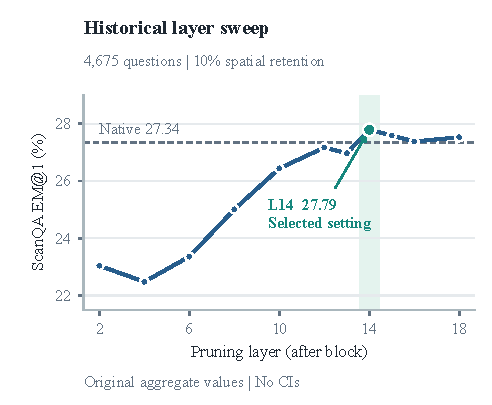
\includegraphics[width=\columnwidth]{fig_layer_curve.pdf}
\caption{Original aggregate ScanQA layer values. The native baseline is 27.34 and L14 is 27.79, without per-question intervals. The main-text paired-replay figure uses its own native 27.4225/L14 27.7219 values and frozen simultaneous contrast intervals. Intervals remain specific to their runner.}
\label{fig:supp_original_layer_curve}
\end{figure}

\subsection{Retention budget}
\label{sec:supp_keep_ratio}

The tested retention ratios yield similar point estimates in the complete 4,675-question sweep at L14 (\Cref{tab:supp_ratio}). Every paired scene-level EM interval relative to the runner-matched baseline includes zero. The default 10\% ratio was chosen from joint validation-set point estimates and is not statistically superior to 5\% or 20\%.

We assess selection stability using a scene-level leave-one-out rule on the same frozen predictions. Each fold selects the budget using the other 70 scenes and evaluates it on the held-out scene. The rule selects 10\% in 68/71 folds. Held-out-selected EM is 27.57, versus 27.79 for fixed 10\%, with a scene-bootstrap difference of $-0.21$ $[-0.50,0.00]$.

\begin{table}[t]
\centering
\caption{Keep-ratio sensitivity on LLaVA-3D ScanQA validation.}
\label{tab:supp_ratio}
\begin{tabular}{lccc}
\toprule
Kept & EM@1 & CIDEr & EM delta 95\% CI \\
\midrule
5\% & 27.72 & 93.12 & [-0.22, 1.01] \\
10\% & 27.79 & 94.33 & [-0.07, 0.99] \\
20\% & 27.68 & 94.32 & [-0.04, 0.73] \\
\bottomrule
\end{tabular}
\end{table}

\subsection{Token-scoring rules}
\label{sec:supp_scorers}

At L14, last-prompt and prompt-mean attention yield higher EM point estimates than the tested random, norm, CLS-attention, and entropy alternatives (\Cref{tab:supp_scorer}). Each scorer is compared at the stated pruning depth. The grid is incomplete, and missing entries are not imputed. A fixed scoring formula can select different token identities across layers, so this comparison does not isolate a depth-only effect.

\begin{table}[t]
\centering
\caption{Scoring-rule comparison at 10\% retention.}
\label{tab:supp_scorer}
\begin{tabular}{lcc}
\toprule
Scorer & L2 EM@1 & L14 EM@1 \\
\midrule
Last-prompt attention & 23.04 & 27.79 \\
Prompt-mean attention & --- & 27.66 \\
Random & 24.77 & 25.67 \\
Token L2 norm & 19.34 & 25.22 \\
CLS attention & 21.22 & 23.23 \\
Attention entropy & --- & 23.23 \\
\bottomrule
\end{tabular}
\end{table}

\subsection{Analytical-cost-matched layer controls}
\paragraph{Selection stability.} Layer selection is stable within the frozen cost-matched runner. Each fold chooses among L2-matched, L8-matched, and L14/128 conditions using the other 70 scenes, then evaluates the selected condition on the held-out scene. L14/128 is selected in 71/71 folds, with a scene-bootstrap selection probability of 0.9984. Nested-selected and fixed-L14/128 EM are both 27.8930, with a difference of 0.0000 $[0.0000,0.0000]$. Unadjusted held-out scene counts are 38/17/16 better/equal/worse for L14 against L2 and 33/17/21 against L8. The scene counts are exploratory.

\paragraph{Scene robustness.} Both prespecified cost-matched contrasts retain positive effects when any complete scene is removed. Using frozen per-question exact-match outcomes, the L14/128 leave-one-scene-out range is $1.0206$--$1.3069$ EM points against L2 and $0.8903$--$1.1206$ against L8. Unadjusted discordant-question counts are 140/83 better/worse against L2 and 144/96 against L8. Their exact two-sided sign-test values are $1.64\times10^{-4}$ and $2.35\times10^{-3}$; Holm correction over the two contrasts gives $3.28\times10^{-4}$ and $2.35\times10^{-3}$. Corresponding scene-mean directions are 38/17/16 and 33/17/21 better/tie/worse.

The sign tests are post-hoc diagnostics and do not replace the prespecified scene-bootstrap intervals for L14/128.

\subsection{Multiplicity within restricted candidate families}
\Cref{tab:supp_max_t} examines selection sensitivity within two frozen three-candidate families. A scene-clustered studentized max-$t$ correction covers all three pairwise contrasts within each family, without reconstructing the complete historical search.

\begin{table*}[t]
\centering
\small
\caption{Limited max-$t$ correction for the frozen layer and budget families. Intervals are 95\% simultaneous intervals over all pairwise contrasts within each stated three-candidate family.}
\label{tab:supp_max_t}
\begin{tabular}{lccc}
\toprule
Family & Contrast & EM points & Max-$t$ 95\% CI \\
\midrule
Layer & L14/128 $-$ L2 cost-matched & $+1.2193$ & $[0.3242,2.1143]$ \\
Layer & L14/128 $-$ L8 cost-matched & $+1.0267$ & $[0.1707,1.8828]$ \\
Layer & L8 cost-matched $-$ L2 cost-matched & $+0.1925$ & $[-0.6284,1.0134]$ \\
Budget & R=0.10 $-$ R=0.05 & $+0.0642$ & $[-0.4565,0.5849]$ \\
Budget & R=0.10 $-$ R=0.20 & $+0.1070$ & $[-0.3317,0.5456]$ \\
Budget & R=0.20 $-$ R=0.05 & $-0.0428$ & $[-0.6353,0.5498]$ \\
\bottomrule
\end{tabular}
\end{table*}

The layer family retains positive intervals after correction, with familywise max-$t$ $p=0.0062$ and critical value 2.3275. The L8-minus-L2 control remains unresolved. All three budget contrasts remain unresolved, with $p=0.8458$ and critical value 2.3286. The two cost-matched L14/128 advantages therefore survive this limited three-candidate correction. R=0.10 remains representative of a quality plateau rather than a unique optimum.

The correction covers only the six listed contrasts, excluding other layers, scorers, budgets, prompts, and thresholds inspected during development. It does not estimate performance under the full historical search.

\subsection{Bootstrap-seed sensitivity}
All six primary paired endpoints retain positive intervals across the tested bootstrap seeds (\Cref{tab:supp_primary_seed}). These endpoints comprise two cost-matched EM contrasts, two first-token log-probability contrasts, and two complete-answer EM contrasts. Each uses the original scene-cluster bootstrap seed and four deterministic offsets, with 10,000 resamples per seed. All six endpoints retain a positive 97.5\% interval under all five seeds, with unchanged point estimates.

\begin{table*}[t]
\centering
\small
\caption{Bootstrap-seed sensitivity for the six primary paired endpoints. The interval range is the union of the five 97.5\% intervals.}
\label{tab:supp_primary_seed}
\begin{tabular}{lccc}
\toprule
Endpoint & Point estimate & Interval range & Stable \\
\midrule
Cost-matched L14$-$L2 EM & 1.2193 & [0.3882, 2.1432] & 5/5 \\
Cost-matched L14$-$L8 EM & 1.0267 & [0.2168, 1.8734] & 5/5 \\
First-token L14$-$L8 & 0.2513 & [0.2108, 0.2965] & 5/5 \\
First-token L14$-$L20 & 0.2159 & [0.1779, 0.2573] & 5/5 \\
Complete-answer L14$-$L8 EM & 3.2014 & [1.7435, 4.7267] & 5/5 \\
Complete-answer L14$-$L20 EM & 2.9733 & [1.8217, 4.2263] & 5/5 \\
\bottomrule
\end{tabular}
\end{table*}

The prespecified seed remains the primary analysis; these post-hoc reruns assess Monte Carlo sensitivity only.

\subsection{Cross-layer scoring and adaptive onset}
Cross-layer score aggregation provides no resolved benefit at the selected L14 configuration. On LLaVA-3D, stable attention obtains 27.55 EM and 93.82 CIDEr, changing EM by $-0.24$ with scene-level 95\% CI $[-0.57,0.10]$. On 3D-LLaVA, windows 2, 3, and 5 likewise have point estimates below single-layer scoring, with intervals containing zero (\Cref{tab:supp_stable}). These comparisons establish neither an improvement nor the absence of an effect.

\begin{table}[t]
\centering
\caption{Stable-attention scoring on 3D-LLaVA ScanQA, L14, 10/100 tokens.}
\label{tab:supp_stable}
\resizebox{\columnwidth}{!}{%
\begin{tabular}{lccc}
\toprule
Scorer & EM@1 & CIDEr & EM delta scene 95\% CI \\
\midrule
Single-layer & 27.83 & 90.42 & --- \\
Window 2 & 27.57 & 89.80 & [-0.64, 0.13] \\
Window 3 & 27.70 & 89.95 & [-0.49, 0.22] \\
Window 5 & 27.66 & 89.80 & [-0.60, 0.26] \\
\bottomrule
\end{tabular}}
\end{table}

Adaptive onset changes pruning depth, but neither variant establishes quality preservation (\Cref{tab:supp_adaptive}). Resetting detector state for each sample produces non-degenerate layer distributions for both variants. The default detector triggers later than fixed L14 on average. The shared detector triggers earlier but has not passed a prespecified non-inferiority test. Historical latency values were collected in separate sessions and are excluded from comparative timing claims.

\begin{table}[t]
\centering
\caption{Corrected adaptive-onset evaluation on LLaVA-3D ScanQA.}
\label{tab:supp_adaptive}
\resizebox{\columnwidth}{!}{%
\begin{tabular}{lcccc}
\toprule
Schedule & Mean layer & Median & EM@1 & CIDEr \\
\midrule
Fixed L14 & 14.00 & 14 & 27.79 & 94.33 \\
Adaptive default & 16.71 & 18 & 27.61 & 94.09 \\
Adaptive shared & 12.75 & 12 & 27.47 & 93.22 \\
\bottomrule
\end{tabular}}
\end{table}

\subsection{Exploratory geometry and coverage}
Both coverage-aware variants score below the attention reference, but their prompt mismatch prevents attributing this difference to the selector (\Cref{tab:supp_coverage}). The selector preserves the highest-attention token, then greedily balances attention against minimum distance to the selected set using OST superpoint centroids. Unit tests verify coordinate alignment, uniqueness, budget clamping, and top-$K$ fallback for invalid coordinates.

Both full-set variants use the original unsuffixed ScanQA prompt. The attention reference uses ``Answer the question simply.'' on the same 4,675 questions. This prompt mismatch prevents interpreting the score differences as paired selector effects. Neither variant is used in GeoGate. The pilot evaluates this greedy selector in the tested 3D-LLaVA runner; it does not reproduce CoVeR's coordinate-covering selector for multi-view 2D VLMs. Its results do not establish that coverage-based selection is generally ineffective.

\begin{table}[t]
\centering
\caption{Unmatched-prompt coverage pilot on 3D-LLaVA ScanQA.}
\label{tab:supp_coverage}
\resizebox{\columnwidth}{!}{%
\begin{tabular}{lccc}
\toprule
Selector & EM@1 & CIDEr & Pairing \\
\midrule
Attention top-$K$ reference & 27.83 & 90.42 & suffixed prompt \\
Stable + coverage, 0.25 & 25.50 & 82.00 & unsuffixed prompt \\
Attention + coverage, 0.10 & 25.48 & 82.45 & unsuffixed prompt \\
\bottomrule
\end{tabular}}
\end{table}

Additional 500-question pilots do not support adopting geometry diffusion or coarsening. Neighbor diffusion overlaps the attention-only pilot range. Mean-pooling discarded tokens into 16 or 64 contiguous or voxel-aware groups yields no point-estimate improvement over deletion and has higher recorded latency. These bounded diagnostics support neither full-set conclusions nor a general absence of benefit.

\section{Task transfer and external evaluation}
\label{sec:supp_transfer}
We evaluate retention quality beyond the ScanQA development comparisons through task transfer, SQA3D validation, and external 3RScan evaluation. These analyses use distinct protocols and decision rules. Attention-pattern persistence is assessed separately from quality outcomes.


\subsection{Five-benchmark quality and multiplicity}
\label{sec:supp_multiplicity}

We assess multiplicity across the five 3D-LLaVA primary endpoints: ScanQA EM, SQA3D EM, Scan2Cap CIDEr@0.25, ScanRefer mIoU, and Multi3DRefer mIoU. This post-hoc analysis uses recorded predictions and 10,000 paired scene-cluster bootstrap resamples per endpoint. Holm step-down correction controls the stated family at $\alpha=0.05$. The official Scan2Cap evaluator contains 2,068 corpus entries: 2,007 have Mask3D predictions, and 61 receive empty hypotheses under the official protocol.

Intervals are marginal percentile intervals rather than simultaneous five-endpoint intervals. Raw two-sided $p$-values use a centered-bootstrap null, defined as the resampled effect minus the observed effect. We count absolute null effects at least as large as the observed effect, with add-one smoothing $(b+1)/(10000+1)$, then apply Holm correction to the five $p$-values.

\begin{table}[t]
\centering
\caption{Family-wise sensitivity across the five 3D-LLaVA primary endpoints. Deltas are GeoGate minus baseline: EM in percentage points, mIoU in 0--100-scale points, and CIDEr in score points. Intervals are marginal paired scene-cluster percentile 95\% intervals; Holm $p$-values address the five-endpoint family.}
\label{tab:supp_multiplicity}
\resizebox{\columnwidth}{!}{%
\begin{tabular}{lcccc}
\toprule
Endpoint & Delta & 95\% CI & Raw $p$ & Holm $p$ \\
\midrule
ScanQA EM & $-0.043$ & $[-0.554,0.503]$ & 0.885 & 1.000 \\
SQA3D EM & $+0.085$ & $[-0.392,0.561]$ & 0.750 & 1.000 \\
Scan2Cap CIDEr@0.25 & $-2.854$ & $[-4.653,-1.081]$ & 0.0011 & 0.0055 \\
ScanRefer mIoU & $-0.143$ & $[-0.289,-0.002]$ & 0.0506 & 0.152 \\
Multi3DRefer mIoU & $-0.318$ & $[-0.504,-0.132]$ & 0.0011 & 0.0055 \\
\bottomrule
\end{tabular}}
\end{table}

The main-text Scan2Cap interval $[-4.68,-1.11]$ is retained from the original per-endpoint analysis reported with seed 20260904. The frozen five-endpoint analysis instead uses Scan2Cap endpoint seed 20260922 and reports $[-4.653,-1.081]$ in \Cref{tab:supp_multiplicity}. These are separate analysis outputs, not alternative rounding of one interval. We retain both with their analysis identities; the available records do not establish that seed alone explains the difference.

The Scan2Cap and Multi3DRefer losses remain resolved after correction (Holm $p=0.0055$ each). ScanRefer's raw bootstrap $p=0.0506$ becomes Holm-adjusted $p=0.1518$, which does not reject the zero-effect null. Neither ScanQA nor SQA3D rejects that null. Percentile intervals are not inversions of the centered-null tests. Thus, ScanRefer's slightly negative interval and raw $p=0.0506$ retain their distinct interpretations without changing the frozen Holm decision. This endpoint correction does not adjust for selecting L14/R=0.10.

The multiplicity decisions persist across the tested bootstrap seeds. We repeat the paired scene-cluster bootstrap with four additional deterministic base seeds. Predictions, scene clusters, endpoint definitions, and the Holm family remain fixed; seed 20260918 remains the primary result. Across all five base seeds, Scan2Cap and Multi3DRefer reject the null in 5/5 runs. ScanQA, SQA3D, and ScanRefer do not reject it in 5/5 runs. Holm $p$ ranges are $[0.0055,0.0100]$ for Scan2Cap, $[0.0040,0.0055]$ for Multi3DRefer, $[0.1518,0.1779]$ for ScanRefer, and exactly 1.0000 for ScanQA and SQA3D. The unchanged decisions support numerical stability across these seeds, while leaving configuration selection and external validity unaddressed.

\paragraph{Precision of the paired intervals.} The QA intervals still permit small losses despite non-rejection of the zero-effect null. Under a normal approximation, we convert each frozen paired scene-cluster interval into an approximate two-sided 80\%-power minimum detectable effect (MDE). The MDEs are 0.779 EM for ScanQA, 0.682 EM for SQA3D, 0.208 mIoU for ScanRefer, 0.266 mIoU for Multi3DRefer, and 2.572 CIDEr for Scan2Cap. In particular, QA non-rejections do not establish equivalence. This post-hoc interpretation describes observed precision rather than a formal power calculation or equivalence test. The scene-clustering, selection, and split-reuse limitations above still apply.

\subsection{SQA3D validation and quality boundaries}
\label{sec:supp_sqa_validation}
The fixed 3D-LLaVA-7B-LoRA L14/R=0.10 configuration was evaluated on all 3,261 official SQA3D validation questions. Fold A contains 1,749 questions from 35 scenes disjoint from development. Fold B contains the remaining 1,512 questions from 30 scenes overlapping ScanQA development. The question partition is answer-blind, but fold B was designed after observing fold A's negative direction. Its subset and non-inferiority rule were then specified before its own outputs. The folds therefore do not constitute a jointly prespecified independent confirmation.

Neither fold overlaps SQA3D train or test scenes. Historical local prediction checks find no exact question-ID matches, but cannot exclude exposure through every checkpoint training source. Both conditions use identical point clouds, the single-word-or-phrase prompt, greedy decoding, seed 0, and a 64-token generation limit.

Before its own generation, each fold's operational non-inferiority margin was fixed at $-1.0$ EM point. Passing requires a one-sided 97.5\% lower scene-bootstrap bound strictly above that margin. \Cref{tab:sqa_validation} reports both completed folds. Intervals use 10,000 scene resamples with seed 20260920. Their two-sided 95\% lower endpoints implement the one-sided decision rule.

\begin{table}[t]
\centering
\caption{SQA3D validation EM changes on 3D-LLaVA. All values are percentage points relative to the paired unpruned baseline.}
\label{tab:sqa_validation}
\small
\begin{tabular}{lrr}
\toprule
Evaluation & $\Delta$ EM & Scene 95\% CI \\
\midrule
Fold A, 35 scenes & $-0.7433$ & $[-1.6609,+0.1170]$ \\
Fold B, 30 scenes & $-1.1905$ & $[-2.0355,-0.4013]$ \\
Combined, 65 scenes & $-0.9506$ & $[-1.5610,-0.3511]$ \\
\bottomrule
\end{tabular}
\end{table}

Neither fold passes the frozen non-inferiority rule. Fold B shows a resolved loss, and the combined interval also excludes zero. The combined estimate summarizes performance across both folds, but fold B's development overlap prevents treating it as independent-domain confirmation. It cannot retroactively change fold A's decision. Both completed failures therefore remain part of the quality boundary.

Post-hoc runs evaluated R=0.05 and R=0.20 on the same folds after these outcomes had been inspected. Combined EM changes are $-0.5826$ $[-1.2584,+0.0628]$ and $-0.4293$ $[-0.8685,+0.0000]$, respectively. Only combined R=0.20 clears the existing $-1.0$ margin. At R=0.20, fold A changes by $-0.0572$ $[-0.6282,+0.5275]$, whereas fold B changes by $-0.8598$ $[-1.5426,-0.2712]$ and still fails the same rule. These post-hoc budget sensitivities provide neither independent confirmation nor a validated safe budget. Combined R=0.20 does not erase the original R=0.10 failures or the exposure from configuration selection.

\subsection{MMScan evaluation on external 3RScan scenes}
\label{sec:supp_mmscan}
\paragraph{Subset and paired protocol.} We evaluate LLaVA-3D-7B on an external subset constructed through label-free overlap checks against the released instruction mixture. Neither of two official MMScan~\cite{lyu2024mmscan} validation-annotation subsets has normalized-question overlap with the released 860K mixture. However, 224 of 803 videos in the larger subset occur there under other tasks: SQA3D, SR3D, Multi3DRefer, Scan2Cap, ScanRefer, NR3D, and ScanQA. Grouping region/view variants by physical scene leaves 246 of 359 base scenes, containing 10,003 questions, with no released-mixture overlap. We freeze the 3RScan portion: 4,934 questions across 234 scenes. A separate exact-match check against the full released mixture finds zero scene-ID, normalized-question, or scene-question pair matches.

The downloaded RGB-D assets pass CRC checks, and all 234 videos pass deterministic preprocessing and input validation. Paired inference runs on one H100 with \texttt{num\_chunks=1}; hardware parallelism is not part of this quality endpoint. Inputs follow the checkpoint's actual 20-frame contract. Baseline and fixed L14/R=0.10 each produce all 4,934 rows and pass structural and scoring-parity checks. Paired scene bootstrap uses 10,000 draws.

\paragraph{Quality result and decision.} The external evaluation does not establish quality superiority. Baseline EM is 11.0053\% and GeoGate EM is 10.9445\%, giving a paired change of $-0.0608$ points with a two-sided 95\% scene-clustered interval $[-0.2980,0.1773]$. CIDEr changes by $-0.2224$ score points $[-1.6586,1.2359]$. The prespecified superiority criterion requires both the EM change and its one-sided 97.5\% lower bound to exceed zero; neither condition is met. The displayed two-sided 95\% interval supplies this lower bound (\cref{sec:supp_statistics}). The EM interval includes zero and does not establish degradation. Non-inferiority was not tested because no loss margin was prespecified; none was introduced retrospectively. The downloaded checkpoint's complete historical training manifest also remains unverified.

\paragraph{Planning assumptions and realized precision.} Before MMScan outputs, a planning calculation scaled inspected ScanQA scene-clustered paired EM variance from 71 to 234 independent scenes. The recorded approximate 80\%-power MDEs are 0.41 and 0.45 EM points. The former uses the standard two-sided 95\% normal cutoff of 1.9600. The latter uses the conservative cutoff 2.2414, rather than the standard one-sided 97.5\% normal quantile. These approximations use no MMScan predictions and do not define the bootstrap decision threshold.

The completed run has scene-bootstrap standard error $0.1213$ EM points. Using the standard normal critical value for a one-sided 97.5\% criterion gives a post-hoc 80\%-power MDE of $0.3397$ EM points. The absolute observed effect is below the prospective 0.45-EM-point and post-hoc MDEs, but that comparison is not a decision rule. This precision summary does not change the superiority criterion or supply an equivalence test.

\paragraph{External attention profiles.} A separately prespecified attention-profile check tests pattern persistence on the same 234 videos. It uses one official question per video in subset order, with the same prompt construction, target clicks, 20-frame contract, and seed. Each video receives one prefill forward pass, without a pruning hook or answer generation. All three scene-clustered criteria are positive: late-minus-middle spatial attention is $+1.5090$ percentage points (95\% scene interval $[1.0888,1.9632]$), the L14--L13 jump is $+7.3029$ points $[6.7963,7.8202]$, and middle-minus-late half-mass coverage is $+3.3986$ points $[2.9841,3.8294]$. The L14--L13 direction is positive for 234/234 videos. These results support external-domain persistence of the attention pattern. They do not test quality preservation, individual-token causality, or the pruning schedule, whose separate quality gate remains inconclusive.

\subsection{Post-hoc profile-to-quality association}
\label{sec:supp_coupling}
Post-hoc association analysis asks whether stronger attention patterns predict quality changes. Profiles and predictions were already inspected before this analysis was specified. For each of 234 3RScan scenes, we compute mean paired L14/R=0.10 EM change and five summaries. These are late-minus-middle attention, L14--L13 attention jump, middle-minus-late half-mass coverage, late half-mass token count, and late received-attention Gini. Pearson and Spearman associations use 10,000 scene-bootstrap resamples and 10,000 label permutations, with Holm adjustment across five endpoints. The primary late-minus-middle endpoint gives Pearson $+0.0790$ $[-0.0730,+0.2729]$ and Spearman $-0.0138$ $[-0.1252,+0.1009]$. It fails the stated same-sign, interval-excluding-zero rule. The raw L14--L13 Spearman estimate is $-0.1337$ $[-0.2596,-0.0044]$, but its Holm-adjusted permutation $p=0.4220$ does not support a relationship after correction. Neither association measure meets its stated decision rule, yielding \emph{no supported monotonic coupling}. This post-hoc diagnostic neither resolves the external quality test nor establishes whether the profile predicts quality under other conditions. Failure to detect a relationship does not establish its absence.

\subsection{Multi3DRefer budget sensitivity}
Increasing the budget reduces the observed Multi3DRefer loss without establishing preservation. We compare frozen 3D-LLaVA predictions at R=10\% and R=20\% with identical prompts, ground-truth object sets, and model identifiers for all 11,120 queries across 141 scenes. \Cref{tab:supp_multi3drefer_budget} reports paired scene-cluster bootstrap 95\% intervals using 10,000 draws.

\begin{table}[t]
\centering
\caption{Multi3DRefer budget sensitivity. Deltas are candidate minus reference in mIoU points on the inspected benchmark.}
\label{tab:supp_multi3drefer_budget}
\resizebox{\columnwidth}{!}{%
\begin{tabular}{lccc}
\toprule
Comparison & Group & Delta & 95\% CI \\
\midrule
R=10\% $-$ baseline & all & $-0.318$ & $[-0.501,-0.134]$ \\
R=20\% $-$ baseline & all & $-0.104$ & $[-0.228,0.018]$ \\
R=20\% $-$ R=10\% & all & $+0.214$ & $[0.092,0.343]$ \\
\midrule
R=20\% $-$ baseline & zero target & $0.000$ & $[-0.333,0.326]$ \\
R=20\% $-$ baseline & one target & $-0.210$ & $[-0.386,-0.039]$ \\
R=20\% $-$ baseline & multiple targets & $+0.149$ & $[-0.002,0.298]$ \\
\bottomrule
\end{tabular}}
\end{table}

The R=20\% point estimate is closer to baseline than R=10\%, with a positive paired R20-minus-R10 difference. The R20-minus-baseline interval includes zero while permitting a loss. By itself, it establishes neither losslessness nor non-inferiority and does not justify recommending a Multi3DRefer budget. Stratified intervals are exploratory and unadjusted for multiplicity. The single-target group has the larger net loss, providing no support for attributing degradation to multi-target queries. We omit an R=30\% sweep because the frozen decision rule required only R=20\% to distinguish a recoverable point estimate from a remaining task boundary.

\section{Measured and analytical efficiency}
\label{sec:supp_efficiency}
We measure LLaVA-3D-7B efficiency under the default GeoGate schedule, distinguishing application time from generation-core timing. Application time decreases by 0.8--1.4\%, whereas generation-core timing and analytical LM estimates cover narrower computational scopes. We report both timing boundaries, followed by tensor-batch throughput and analytical LM cost. \Cref{fig:supp_original_teaser} summarizes these distinct measurements, which do not establish quality superiority at matched measured cost.

\begin{figure*}[t]
\centering
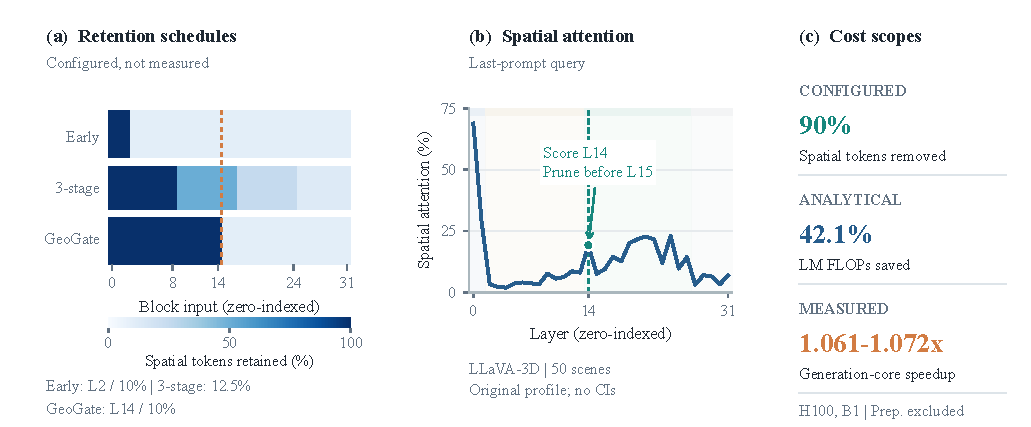
\includegraphics[width=\textwidth]{fig_teaser.pdf}
\caption{Tested schedule and distinct evidence scopes. Retention schedules, attention profiles, analytical LM cost, and measured generation speed describe different quantities. Their juxtaposition establishes neither matched-cost quality dominance nor independent quality preservation.}
\label{fig:supp_original_teaser}
\end{figure*}

\subsection{Generation and application time at batch size one}
Each batch-size-one session loads both conditions once and alternates their order across questions. It uses ten warm-up questions and synchronizes CUDA around generation, with inputs GPU resident when timing begins. \Cref{tab:supp_b1} reports the three full-set sessions separately.

\begin{table}[t]
\centering
\caption{Paired generation-core timing on one H100, batch size one. Times in milliseconds are condition-wise medians. The ratio is the median of paired per-question GeoGate/native times, not the quotient of the two medians.}
\label{tab:supp_b1}
\begin{tabular}{lccc}
\toprule
Session & Native & GeoGate & Paired ratio \\
\midrule
1 & 160.20 & 150.60 & 0.9429 \\
2 & 159.98 & 150.41 & 0.9411 \\
3 & 144.97 & 135.13 & 0.9324 \\
\bottomrule
\end{tabular}
\end{table}

Generation-core ratios correspond to reciprocal speedups of $1.061\times$, $1.063\times$, and $1.072\times$. Broader application-time ratios are 0.9921, 0.9910, and 0.9855, representing reductions of 0.8--1.4\%. This broader boundary includes preprocessing, transfer, generation, and decoding. Median allocation increments decrease from 1,613 to 1,052 MiB, excluding parameters and inputs that are already resident.

\subsection{Same-scene tensor batches}
The B2/B4 runs (\Cref{tab:supp_batch}) use tensor batches of questions from the same scene and include remainder-padding time in the useful-throughput denominator. Three fresh processes each evaluate all 4,675 questions. Validation covers 18,972 raw rows, 3,569 multimodal preparations, and 7,138 model calls; all checks pass in every process.

\begin{table*}[t]
\centering
\caption{Controlled same-scene tensor-batch throughput on one H100. Each useful q/s value is the real-question count divided by summed batch generation time, including padding time. The throughput ratio is native total time divided by GeoGate total time; intervals target this ratio.}
\label{tab:supp_batch}
\begin{tabular}{cccccc}
\toprule
Batch & Session & Native useful q/s & GeoGate useful q/s & Total-time ratio & Scene 95\% CI \\
\midrule
2 & 1 & 5.548 & 6.189 & 1.115 & [1.101, 1.130] \\
2 & 2 & 5.456 & 6.056 & 1.110 & [1.094, 1.125] \\
2 & 3 & 5.469 & 6.063 & 1.109 & [1.094, 1.123] \\
4 & 1 & 6.559 & 7.691 & 1.172 & [1.155, 1.189] \\
4 & 2 & 6.679 & 7.893 & 1.182 & [1.165, 1.198] \\
4 & 3 & 6.589 & 7.755 & 1.177 & [1.160, 1.193] \\
\bottomrule
\end{tabular}
\end{table*}

All 4,675 EOS-trimmed outputs reproduce exactly across processes within each batch-size/condition cell. GeoGate does not generate shorter answers: mean lengths increase by 0.021 tokens at B2 and 0.047 at B4, while medians and P95 values are identical. These results measure GPU-resident generation with homogeneous same-scene batches, rather than end-to-end serving.

\subsection{Mixed-scene heterogeneous batches}
The v18c follow-up (\Cref{tab:supp_hetero_batch}) tests heterogeneous batching while keeping the frozen model, prompts, seed, B4 schedule size, and generation-core timing boundary. Three fresh processes each evaluate all 4,675 questions. Among 1,169 batches, 1,168 contain at least two scenes and at least two visual-token counts. The predeclared terminal remainder contains three real questions and one padding slot.

Each batch's elapsed time, including padding, is divided equally among its real questions. Summing these allocations over the full set counts each batch time exactly once. The total-time ratio therefore compares native and GeoGate generation-core time under the recorded schedule. The displayed rates instead summarize median allocated time per question.

\begin{table*}[t]
\centering
\caption{Mixed-scene heterogeneous B4 generation on one H100. The rate columns (q/s) are reciprocals of condition-wise median allocated time per real question. The total-time ratio instead divides summed native allocated times by summed GeoGate times. Frozen scene intervals refer to this ratio under the allocation-based procedure; coverage for shared batch timing and between-session variation remains unvalidated. Dividing the displayed rate columns does not recover the ratio.}
\label{tab:supp_hetero_batch}
\begin{tabular}{cccccc}
\toprule
Session & Native rate & GeoGate rate & Total-time ratio & Scene 95\% CI & Mean length delta \\
\midrule
1 & 5.557 & 6.065 & 1.088 & [1.082, 1.094] & +0.0077 \\
2 & 5.532 & 6.053 & 1.091 & [1.084, 1.098] & +0.0015 \\
3 & 5.651 & 6.181 & 1.091 & [1.084, 1.098] & +0.0077 \\
\bottomrule
\end{tabular}
\end{table*}

The frozen bootstrap samples scenes jointly for native and GeoGate, preserving question pairing and each scene's question group. However, the 1,168 mixed batches share measured times across scenes. Scene resampling can give different multiplicities to portions of the same batch time, so it does not preserve batch-level timing dependence. We retain these intervals as scene-reweighting summaries conditional on the recorded schedule and allocation. Their coverage for execution-time variation has not been established; the per-session intervals also do not estimate between-process uncertainty. This limitation establishes neither the direction nor the magnitude of any interval-coverage error.

All three sessions meet the throughput criterion under the recorded decision procedure. GeoGate has identical median and P95 answer lengths, and its mean length is not shorter. However, 73 of 18,700 question-condition pairs differ across processes despite matching input-tensor hashes for all 9,352 slots. Exact output reproduction across processes is therefore not established.

A bounded repeat diagnostic examines eight batches from the three scenes exceeding the 2,560-token preparation cap. Each condition order is repeated three times, comparing EOS-trimmed token sequences. Input-tensor hashes and GeoGate pruning traces match, but 15 of 32 condition-order groups produce multiple sequences (6 baseline and 9 GeoGate groups). This demonstrates non-bitwise generation within the tested runner, beyond cross-process or condition-order differences. Backend isolation repeats seven of these batches: native SDPA with GPU scatter yields 13/28 stable same-order groups, math SDPA 13/28, eager attention 12/28, and ordered CPU-reference voxel scatter 13/28. Inputs and pruning traces match throughout. The instability is therefore not isolated to these attention or scatter kernels.

Post-hoc exclusion of the 58 questions with any cross-process mismatch leaves 4,617 questions per session. Throughput ratios remain $1.088$--$1.092$, with frozen scene lower bounds above $1.082$. This calculation retains parts of some batch-time allocations; it does not measure a rerun of the smaller workload. It therefore shares the interval-dependence limitation above. The recorded throughput rule uses per-batch timing and does not require bitwise output identity. These ratios characterize generation-core throughput in the evaluated sessions, without establishing token determinism, quality equivalence, or end-to-end serving speedup.

\subsection{Analytical LM cost and decode length}
The analytical LM proxy uses hidden width $d=4096$, feed-forward width $I=11008$, and $L=32$ decoder blocks. Per-layer prefill cost is $f(s)=4sd^2+2s^2d+3sdI$; one-step decode cost is $h(k)=4d^2+2kd+3dI$. GeoGate prefills 15 full-length and 17 reduced-length blocks. After all-layer prompt-cache compaction, the decode proxy uses $k=T_{\text{kept}}=370$ at every block, versus $T=1717$ for native. Cache lengths remain fixed throughout the assumed decode steps, excluding generated-token growth. The KV ratio $370/1717$ therefore estimates prompt storage at decode initialization, not final answer-cache size. Vision, token selection, cache indexing, and total GPU allocation lie outside this analytical model.

The reported analytical ratio assumes eight decode steps. \Cref{tab:supp_cost_sensitivity} evaluates the same equations for one through 32 steps. The machine-readable results also include mean generation lengths from the three frozen timing sessions. This sensitivity analysis concerns analytical LM cost, not measured latency or full-model FLOPs.

\begin{table}[t]
\centering
\caption{Analytical LM cost ratios across decode lengths.}
\label{tab:supp_cost_sensitivity}
\resizebox{\columnwidth}{!}{%
\begin{tabular}{rccc}
\toprule
Decode steps & GeoGate ratio & GeoGate reduction & FastV minus GeoGate \\
\midrule
1 & 0.5776 & 42.24\% & 1.28 pp \\
2 & 0.5778 & 42.22\% & 1.28 pp \\
4 & 0.5783 & 42.17\% & 1.28 pp \\
8 & 0.5791 & 42.09\% & 1.28 pp \\
16 & 0.5808 & 41.92\% & 1.29 pp \\
32 & 0.5842 & 41.58\% & 1.30 pp \\
\bottomrule
\end{tabular}}
\end{table}

GeoGate's analytical LM cost reduction stays within $41.58$--$42.24\%$ across this range. The FastV L2/R50 total-cost gap remains $1.28$--$1.30$ percentage points. The prefill ratio, $0.5774$, does not depend on the assumed decode budget.

\section{Baseline context and reproducibility}
\label{sec:supp_repro}
This section defines the scope of the baseline comparisons and identifies the assets needed to inspect or reproduce the results. Statements about implementation availability apply to the inspected repository commits, not necessarily to current releases.


\subsection{Reproduction scope}

Rebuilding the document, inspecting saved records, rescoring predictions, and replaying inference require different assets. \Cref{tab:supp_repro_scope} identifies the available inputs and remaining requirements for each activity. A matching hash establishes content identity with the recorded file; it does not verify historical execution or complete runtime availability.

\begin{table*}[t]
\centering
\caption{Reproduction scope of the accompanying document package and indexed local records. The source bundle supports document rebuilding; it is not a standalone experimental release.}
\label{tab:supp_repro_scope}
\begin{tabular}{@{}>{\raggedright\arraybackslash}p{0.18\textwidth}>{\raggedright\arraybackslash}p{0.37\textwidth}>{\raggedright\arraybackslash}p{0.39\textwidth}@{}}
\toprule
Activity & Available inputs & Verification boundary \\
\midrule
Document rebuilding & TeX, styles, references, and figure PDFs in the package &
The document can be compiled without model inference. \\
Record inspection & Local predictions, ground truth, question inputs, and indexed sources &
Selected copies match recorded hashes; known source mismatches remain indexed.
Indexed files need not be publicly redistributed. \\
Prediction rescoring & Saved answers and a hash-matching scoring entry &
The scorer was not rerun for this revision; full dependencies and numerical parity remain unvalidated. \\
Inference replay & Hash-matching historical GeoGate core and four upstream model files &
The historical quality runner remains unretrieved; complete model, data, import, and runtime dependencies remain unvalidated. \\
\bottomrule
\end{tabular}
\end{table*}

\subsection{Project-relative entry points}
\label{sec:supp_repro_index}

\Cref{tab:supp_repro_entries} locates existing experiment records in the project checkout. Paths are relative to the project root, with \texttt{A} denoting \texttt{analysis/}, \texttt{G} denoting \texttt{adaptive\_token/}, and \texttt{F} denoting \texttt{results/raw/followup/}. These are local artifact pointers, not public download links. The accompanying \nolinkurl{REPRODUCTION_INDEX.md} lists complete paths, model dependencies, availability checks, and known source-version gaps; \nolinkurl{repro_evidence.json} records file hashes and evidence locations from the earlier inspection. \nolinkurl{provenance_recovery_20261104.json} records the additional local hash matches described below.

\begin{table*}[t]
\centering
\caption{Project-relative reproduction pointers. Each row identifies a code entry and its frozen record; it does not certify a complete runnable release. Full paths and additional endpoints appear in the accompanying index.}
\label{tab:supp_repro_entries}
\begin{tabular}{@{}>{\raggedright\arraybackslash}p{0.15\textwidth}>{\raggedright\arraybackslash}p{0.38\textwidth}>{\raggedright\arraybackslash}p{0.41\textwidth}@{}}
\toprule
Evidence & Existing entry & Record or configuration \\
\midrule
Attention profiles & \nolinkurl{A/e1_attention_profile.py};
\nolinkurl{A/e1b_attention_profile_3dllava.py} &
\nolinkurl{results/raw/e1_profile_llava3d.json};
\nolinkurl{results/raw/e1b_profile_3dllava.json} \\
Matched-input QA & \nolinkurl{G/run_shared_input_quality_v3.py} &
\nolinkurl{F/review_v3_20260908/quality_full.manifest.json} \\
Analytical-cost controls & \nolinkurl{G/run_stage_v4.py} &
\nolinkurl{F/review_v4_audit_20260910/manifest.json} \\
Paired layer replay & \nolinkurl{G/run_layer_sweep_paired.py} &
\nolinkurl{F/layer_sweep_paired_20260920/layer_sweep_audit.json} \\
Readout controls & \nolinkurl{A/run_readout_generation_v15.py};
\nolinkurl{A/run_fixed_deletion_v21.py} &
\nolinkurl{F/readout_generation_v15_full_20260913/full.manifest.json};
\nolinkurl{F/fixed_deletion_v21_full_20260917/full.manifest.json} \\
Timing and batching & \nolinkurl{G/run_scanqa_timing_boundaries_v4.py};
\nolinkurl{A/run_hetero_batch_throughput_v18.py} &
\nolinkurl{F/timing_boundaries_v5_20260912/outputs/session1.manifest.json};
\nolinkurl{F/hetero_batch_v18b_throughput_mixed_b4_20260919/summary_v18c_independent.json} \\
SQA3D validation & \nolinkurl{G/run_sqa3d_scene_disjoint.py} &
\nolinkurl{F/sqa3d_scene_disjoint_20260919/manifest.json};
\nolinkurl{F/sqa3d_validation_replication_20260919/manifest.json} \\
External 3RScan & \nolinkurl{G/run_mmscan_geogate.py} &
\nolinkurl{F/mmscan_3rscan_confirmation_20260917/experiment_lock_v2.json} \\
\bottomrule
\end{tabular}
\end{table*}

\paragraph{Model and source identities.} The records identify \texttt{LLaVA-3D-7B}, and \texttt{3D-LLaVA-7B-LoRA} with the \texttt{llava-v1.5-7b} base and \nolinkurl{ost-sa-only-llava-align-scannet200.pth} point-cloud weights. \nolinkurl{results/PUBLICATION_PROVENANCE_20260916.json} records checkpoint, adapter, base-model, and point-cloud file hashes. These identities were read from local records; remotely stored weights were not revalidated. The matched-input QA runner still differs from its historical manifest hash. The historical core's matching copies are indexed under \nolinkurl{F/adaptive_corrected_v2_20260912/adaptive_token/geogate_v0.py} and \nolinkurl{F/timing_boundaries_v5_20260912/adaptive_token/geogate_v0.py}. Inference replay additionally requires complete authorized model/data assets and the environment described in the index.


\paragraph{Run identities and integrity checks.} The shared-input complete-answer run, \texttt{v15}, contains 74,800 JSONL rows for 4,675 questions under 16 conditions. The fixed-set replay, \texttt{v21}, reproduces its unpruned baseline exactly (\texttt{mismatch\_count=0}). The MMScan input preflight corrected a stale 24-frame expectation to the checkpoint's actual 20-frame contract.

\paragraph{Fixed-set factorial diagnostic.} Machine-readable result: \texttt{results/raw/followup/}\allowbreak \texttt{fixed\_deletion\_v21\_full\_20260917/}\allowbreak \texttt{factorial\_decomposition\_20260918.json}; implementation: \texttt{analysis/}\allowbreak \texttt{audit\_fixed\_deletion\_v21\_factorial.py}.


\subsection{Related methods and baseline availability}
\label{sec:supp_baseline_availability}

\textbf{Broader related work.} Related 3D interfaces cover embodied action, generation, object understanding, and interactive grounding~\cite{huang2024leo,zhen20243dvla, qi2024gpt4point,qi2024shapellm,chen2024ll3da,chen2024grounded3dllm}, building on alignment and open-vocabulary perception~\cite{zhou2023uni3d, xue2023ulip,peng2023openscene,jatavallabhula2023conceptfusion}. EViT, ToMe, SparseVLM, VisPruner, and FoPru study reorganization, merging, or importance selection outside the tested 3D protocol~\cite{liang2022evit, bolya2023tome,zhang2024sparsevlm,zhang2024fastervlm,jiang2024fopru}. DINO and TokenLearner provide related analyses of attention and token structure~\cite{caron2021dino,ryoo2021tokenlearner}. HiMAP studies information flow and hierarchical pruning~\cite{yin2025himap}, establishing phase-based pruning as an existing research direction. GeoGate contributes measurements in 3D models and controls that delimit the scheduling interpretation.

\paragraph{HiSC.} The official HiSC repository was checked at the following commit:
{\raggedright\par\noindent
\texttt{a9b2ee51df8bee0f6c21\allowbreak fc7e1852f00a7f2e81b3}.\par}
At that commit, it contained only a two-line README and provided no executable model, configuration, checkpoint binding, or evaluation entry point. HiSC therefore remains directly related work; we claim no official reproduction and include no self-reported metrics in the implemented-baseline table.

\paragraph{CoVeR.} The official CoVeR project links to the repository and checked commit below:
{\raggedright\par\noindent
\url{https://github.com/humansensinglab/CoVeR}\par\noindent
\texttt{45c9865cb45121802d5e\allowbreak ba144f20d4da4a126624}.\par}
At that commit, its README stated that the full codebase is forthcoming. The repository provides no executable selector, model configuration, checkpoint binding, or evaluation entry point. We discuss CoVeR as directly related work without an implemented baseline or empirical comparison. The superpoint coverage experiment is not a CoVeR reproduction.

\paragraph{HCC-3D.} The official HCC-3D repository was checked at the following commit:
{\raggedright\par\noindent
\texttt{9017e87342d4e17ecd75\allowbreak d9419bdea3b7053e99f5}.\par}
It releases training and evaluation code with model checkpoints for a PointLLM/Phi-2 object understanding stack. It evaluates ModelNet40 classification and Objaverse classification and captioning. Its learned compressor, checkpoint, input representation, and task protocol are incompatible with our frozen LLaVA-3D ScanQA and SQA3D pipelines. We therefore discuss HCC-3D as related work without placing its self-reported metrics in the implemented-baseline table.

\subsection{Recorded environment and checksums}
Key frozen artifact hashes are:

\begin{itemize}
\item complete-answer intervention raw JSONL: \texttt{23591076458c4626}\allowbreak \texttt{908f3a16b955400f}\allowbreak \texttt{83aec77b8f72752f}\allowbreak \texttt{47e058e81690d33a};
\item first-token intervention raw JSONL: \texttt{30324c06a4d20883}\allowbreak \texttt{dadd9ceeb876321e}\allowbreak \texttt{02b52d8784cf8370}\allowbreak \texttt{422a1a1100a897fa};
\item matched-input quality raw JSONL: \texttt{426cb1bd5c828562}\allowbreak \texttt{7a182faddff476cc}\allowbreak \texttt{81a5e6fd81b98a16}\allowbreak \texttt{4ae66136c2ad9ff9};
\item deterministic tensor-batch final comparison: \texttt{2c8613b36da2d0c6}\allowbreak \texttt{b0ae775c748b4af0}\allowbreak \texttt{320d5729abadad4f}\allowbreak \texttt{3b592d02a59895c6}.
\end{itemize}

Execution records identify Python 3.10.20, PyTorch 2.6.0 with CUDA 12.4, cuDNN 9.1, Transformers 4.37.2, and driver 580.95.05 on one H100 80GB. These versions document the completed runs; they were not prespecified experimental factors.

\section{Qualitative answer transitions}
\label{sec:supp_qualitative}
% Questions, references, answers, and original table bodies remain frozen.
\label{sec:supp_answer_cases}

\Cref{tab:supp_cases_a,tab:supp_cases_b} illustrate each exact-match transition with one example from each frozen SQA3D validation fold. Within each fold and outcome, selection uses the smallest SHA256 of \texttt{geogate-v80-case|fold|question\_id}. This rule was fixed before reading the selected texts, after the original experiment. Every eligible question entered selection; length, visual appeal, and error severity were not filters. Answers use evaluator normalization, while the full situation, question, answer-format suffix, and raw references remain unchanged.

Each \emph{eligible} count is the total number of questions in that fold's exact-match transition category. These counts describe the observed folds; the eight selected examples do not estimate frequencies beyond those folds. They illustrate output transitions without identifying semantic causes, visual mechanisms, or individual-token causality.

Fold A's wrong-to-correct example changes ``l shaped'' to the reference ``l-shaped''. Its wrong-to-wrong example answers ``picture'' against ``pictures''. Both illustrate exact-match sensitivity to wording, rather than demonstrated semantic improvement or deterioration. Fold B includes directional (left/right) and color (brown/red) transitions. Answers alone do not reveal the causes of these changes.

\begin{table*}[p]
\centering
\small
\caption{Fixed-rule SQA3D examples, fold A: development-disjoint scenes. No case is selected by visual inspection.}
\label{tab:supp_cases_a}
\begin{tabular}{@{}p{0.13\textwidth}p{0.51\textwidth}p{0.14\textwidth}p{0.14\textwidth}@{}}
\toprule
Transition & Situation and question / reference & Native & GeoGate \\
\midrule
Wrong to correct\newline 22 eligible & I set my coffee cup down on the table and there is a couch to my right. What shape is the red couch to my 3 o'clock? Answer the question using a single word or phrase.\newline \textit{Reference:} l-shaped\newline {\footnotesize val-scene0568\_00-19} & l shaped & l-shaped \\
\midrule
Correct to wrong\newline 35 eligible & I am facing a mattress across the room and there is a cabinet on my right. Is the number of pictures in front of me odd or even? Answer the question using a single word or phrase.\newline \textit{Reference:} even\newline {\footnotesize val-scene0629\_00-43} & even & odd \\
\midrule
Correct to correct\newline 937 eligible & I am in front of the whiteboard getting ready for a meeting in 15 minutes, and right behind me is a table with a chair in the corner of the table. Is the amount of whiteboard I am facing odd or even? Answer the question using a single word or phrase.\newline \textit{Reference:} odd\newline {\footnotesize val-scene0655\_00-11} & odd & odd \\
\midrule
Wrong to wrong\newline 755 eligible & I am placing can bottles into the recycling bin in front of me, fridge is to my right. What's on the wall behind me? Answer the question using a single word or phrase.\newline \textit{Reference:} pictures\newline {\footnotesize val-scene0670\_00-2} & picture & picture \\
\bottomrule
\end{tabular}
\end{table*}

\begin{table*}[p]
\centering
\small
\caption{Fixed-rule SQA3D examples, fold B: development-overlapping scenes. No case is selected by visual inspection.}
\label{tab:supp_cases_b}
\begin{tabular}{@{}p{0.13\textwidth}p{0.51\textwidth}p{0.14\textwidth}p{0.14\textwidth}@{}}
\toprule
Transition & Situation and question / reference & Native & GeoGate \\
\midrule
Wrong to correct\newline 12 eligible & I sit at the head of the table and around me are other chairs. Which direction should I go if I want to open the window? Answer the question using a single word or phrase.\newline \textit{Reference:} right\newline {\footnotesize val-scene0011\_00-21} & left & right \\
\midrule
Correct to wrong\newline 30 eligible & I started cooking at the kitchen island and behind me was the kitchen counter. What color is the chair that is facing the table in front of me to left? Answer the question using a single word or phrase.\newline \textit{Reference:} brown\newline {\footnotesize val-scene0063\_00-34} & brown & red \\
\midrule
Correct to correct\newline 804 eligible & I am holding on a chair in my ten o'clock direction, standing between two tables. I hear the phone ringing in a backpack on my right. I can easily pick the backpack by stretching my right hand: true or false? Answer the question using a single word or phrase.\newline \textit{Reference:} true\newline {\footnotesize val-scene0196\_00-18} & true & true \\
\midrule
Wrong to wrong\newline 666 eligible & I am standing between a table and a whiteboard, while there is a backpack in my one o'clock direction. Is the space that I can move forward from my current direction? Answer the question using a single word or phrase.\newline \textit{Reference:} yes\newline {\footnotesize val-scene0342\_00-33} & no & no \\
\bottomrule
\end{tabular}
\end{table*}


\clearpage

\section{Limitations and remaining validation}
\label{sec:supp_limitations}

Both tested models use Llama-family 7B language backbones, limiting the architectural scope of the evidence. The experiments establish neither a universal L14 boundary, a mechanism unique to 3D inputs, nor individual-token causality. Independent quality preservation is not established: the SQA3D development-disjoint fold fails non-inferiority, combined validation shows a loss, and MMScan fails its superiority criterion. Systems measurements cover one H100 under controlled same-scene and mixed-scene generation-core batching. Mixed-scene interval coverage remains unvalidated for shared batch timing and between-process variation. The tested geometry, temporal-aggregation, and adaptive-onset variants yield negative or unresolved results. These findings delimit the tested schedule rather than establishing general limits of token pruning.

\subsection{Remaining validation requirements}
\label{sec:supp_pending}
\paragraph{OpenEQA-HM3D.} OpenEQA~\cite{majumdar2024openeqa} is the planned independent preservation test; other independent evaluation designs remain possible. Its frozen eligibility check identifies 557 official questions across 63 HM3D episodes. The recorded asset check passes 0/63 episodes because the inspected workspace lacks episode RGB frames; the check is not an exhaustive asset inventory. Evaluation requires authorized complete RGB-D frames, poses, intrinsics, and a usable frozen official LLM-Match scorer. EM/F1 remain auxiliary endpoints and cannot replace the protocol's primary preservation test.

\paragraph{Complete three-condition quality--cost comparison.} The native/GeoGate timing sessions already record paired answers and quality. The remaining requirement is a matched joint comparison with official 3DZip, including complete preparation-plus-generation time. The existing official-3DZip quality study and native/GeoGate timing sessions use separate runners and cannot form that three-condition Pareto comparison. A prospective protocol must measure answers and actual times for native, official 3DZip, and GeoGate together, including vision/compression and selection/cache work. This requirement is distinct from the independent preservation test above.


{
    \small
    \bibliographystyle{ieeenat_fullname}
    \bibliography{main}
}
\end{document}
